\documentclass[11pt]{article}

\usepackage{graphicx}
\usepackage{glossary}
\usepackage{url}
\usepackage{xspace}

\graphicspath{{figures/}}


\newcommand{\JUnit}{\textsc{JUnit}\xspace}
\newcommand{\JExample}{\textsc{JExample}\xspace}

\newcommand{\ttt}[1]{\texttt{#1}}


%%%%%%%%%%%%%%%%%%%%%%%%%%%%%%%%%%%%%%%%%%%%%%%%%%%%%%%%%%%%
\begin{document}

\title{JExample}

\author{Lea H\"ansenberger\\
	Supervised by: Adrian Kuhn\\
	University of Bern, Switzerland\\
	Software Composition Group
}

\maketitle

\begin{abstract}

\end{abstract}

%%%%%%%%%%%%%%%%%%%%%%%%%%%%%%%%%%%%%%%%%%%%%%%%%%%%%%%%%%%%
\section{Introduction}
 
\section{Related Work}

\section{Example}

\section{Implementation}

To extend the \JUnit Framework mainly one class is needed. The Runner. This class consists of three parts corresponding to the three steps of a test run.

\begin{enumerate}
 \item a constructor for the initialization of the Runner
 \item a method \verb|Runner.run()| to run the test methods
 \item a method \verb|Runner.getDescription()| to get information about the run
\end{enumerate}

For \JExample also wrapper classes and validators needed to be adapted. \JUnit only allows methods without parameters and with return type void. As methods in \JExample need to be allowed to take arguments and return objects, the validation of the methods needed to be adapted.

See Figure \ref{fig:classDiag} for the important classes of the extension.


\begin{figure}[htbp]
 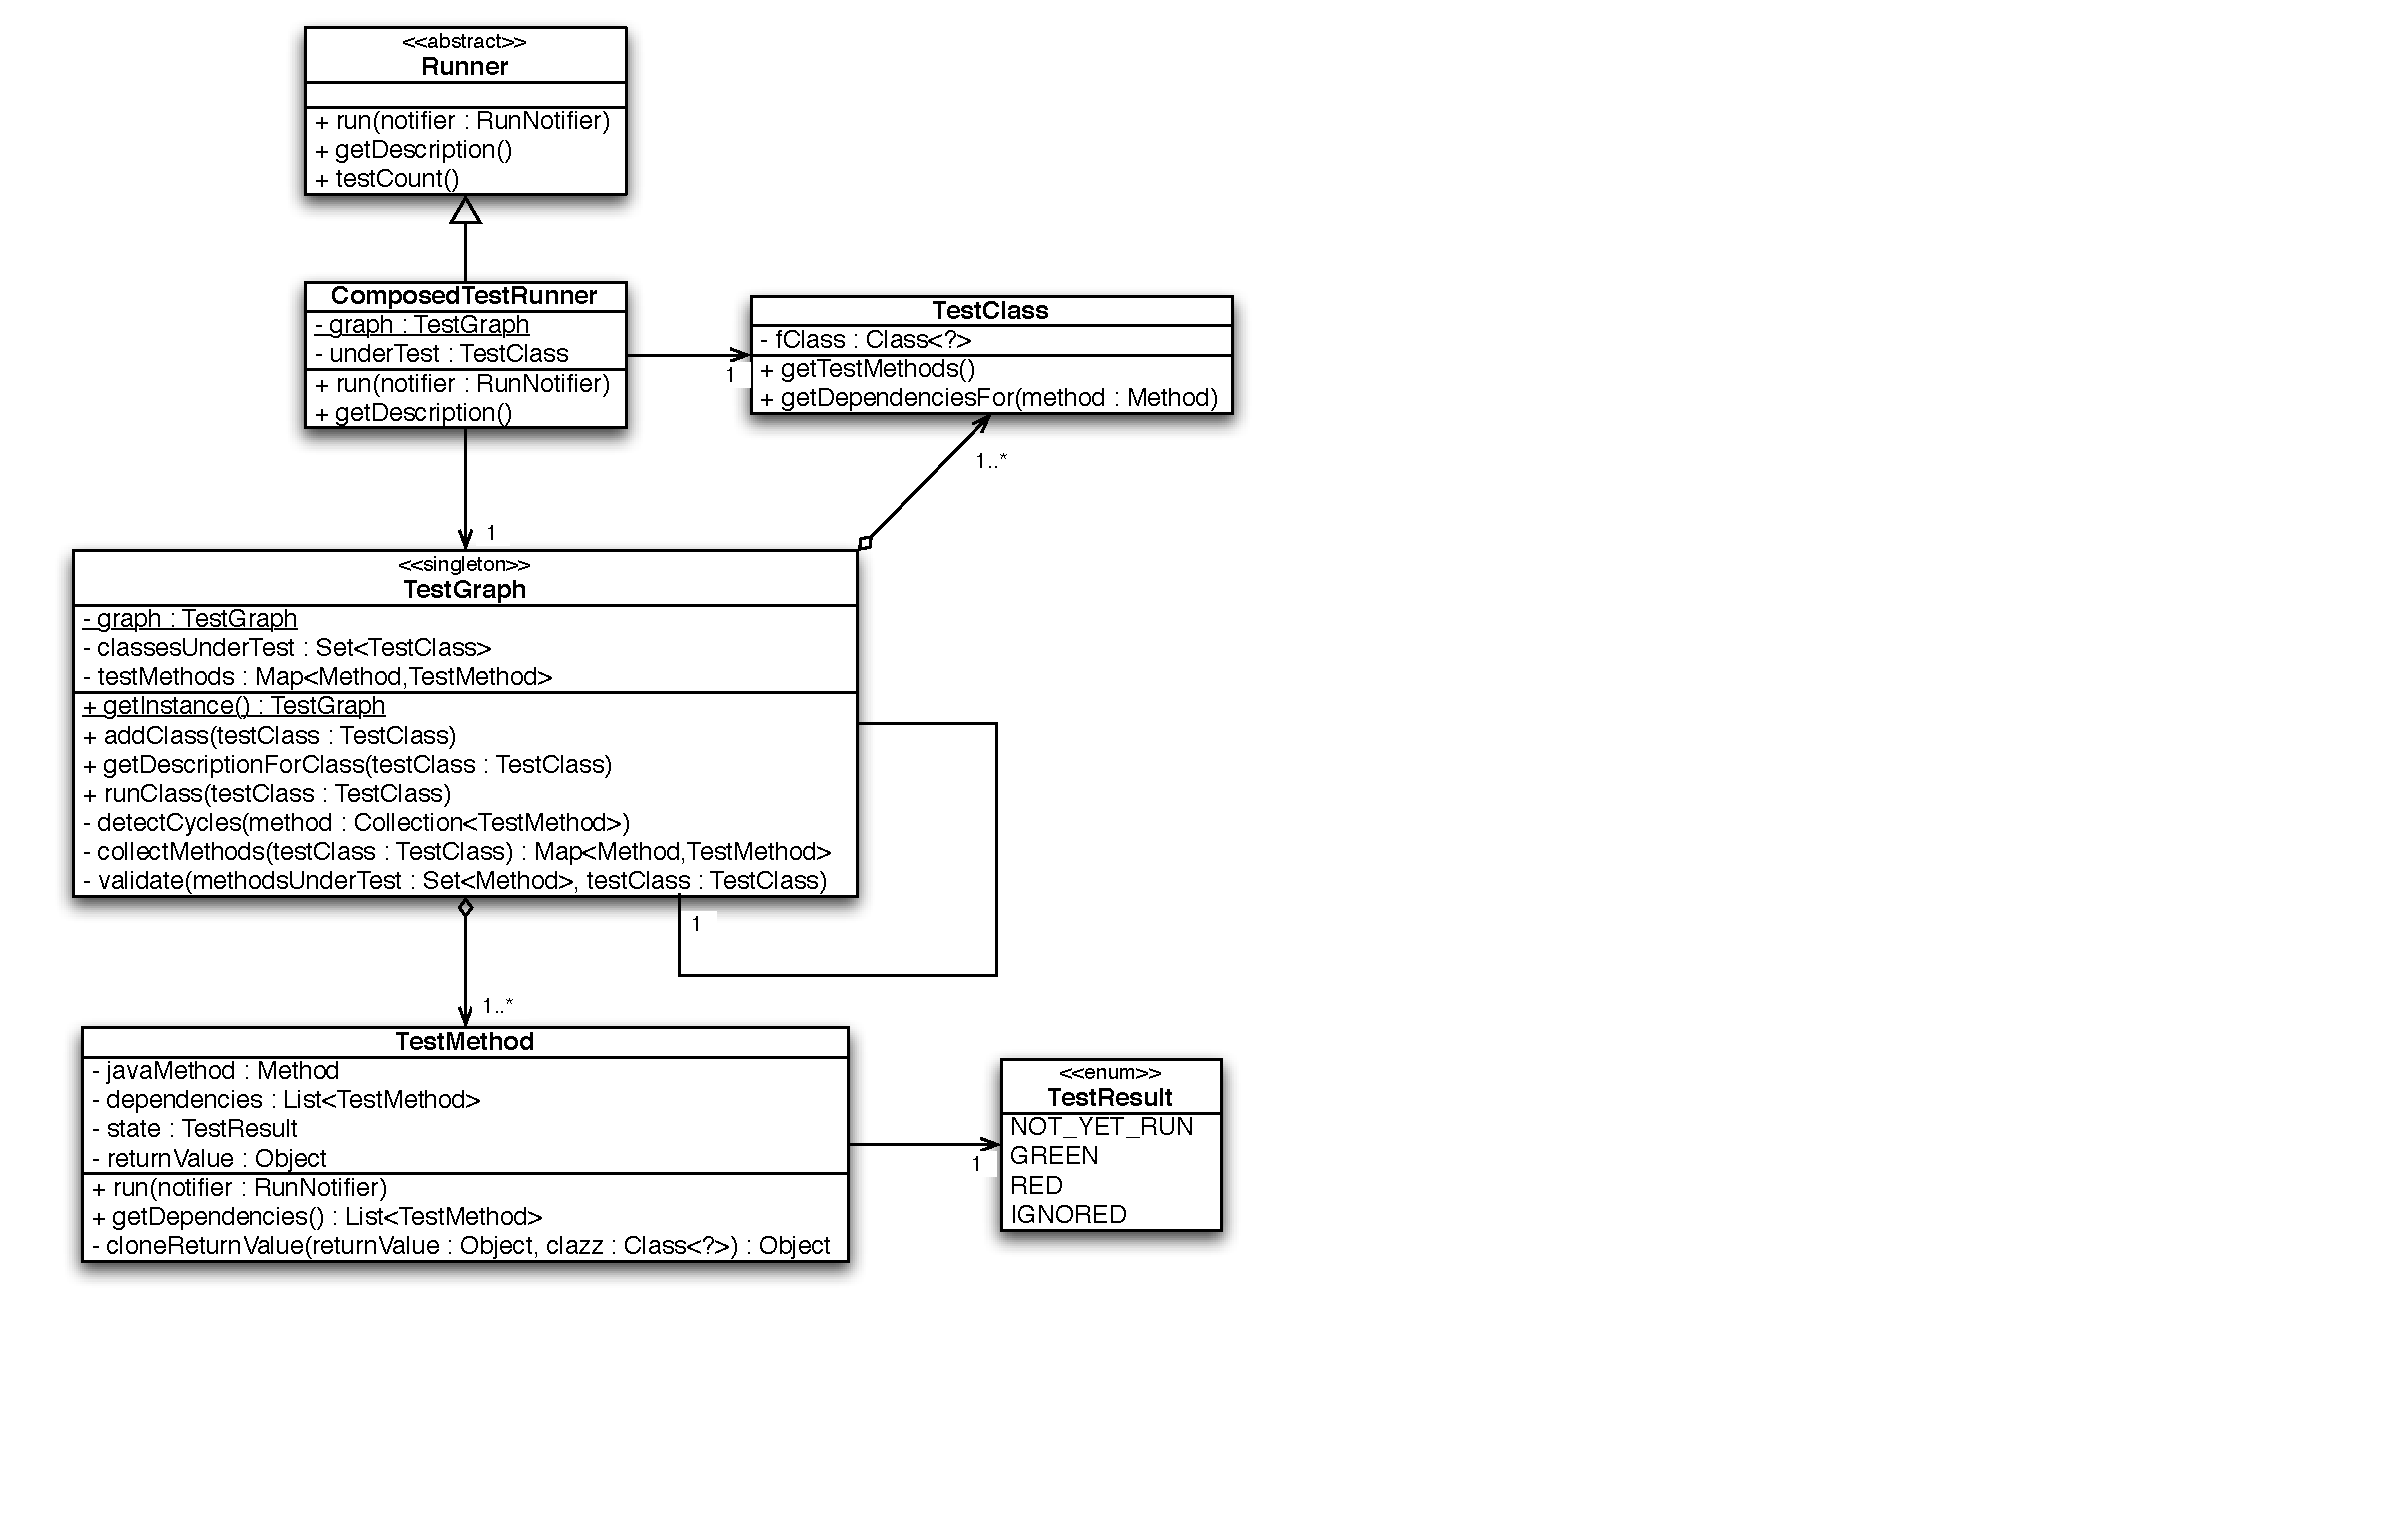
\includegraphics[width=24.0cm]{classdiagram.pdf}
 \caption{Class Diagram}
 \label{fig:classDiag}
\end{figure}


\subsubsection{The Runner}

The Runner is the main connection to the \JUnit Framework, in this case this is the \verb|ComposedTestRunner|. It extends the abstract class \verb|org.junit.runner.Runner| and implements two methods \verb|Runner.run()| and \verb|Runner.getDescription()|. A test run consists of three steps:
\begin{enumerate}
 \item initializing the Runner, this includes collecting and validating methods and test dependencies
 \item running the methods
 \item getting the description of the run
\end{enumerate}

\subsubsection{The TestGraph}

The actual Runner in the extension is the \verb|TestGraph|. The reason for delegating this responsibility to another class is that we wanted the Runner to be a singleton. A singleton is necessary because a method can depend on a method from another class. It makes sure, that every method is collected and run only once in a test run and therefore only counted once so the run count correpsonds to the number of methods.

The \verb|TestGraph| reflects the three steps in its three public methods \verb|addClass()| for the initialization, \verb|runClass()| for running the methods and \verb|getDescriptionForClass()| for getting the description of all the run methods. If methods declare dependencies to methods of other classes, those dependencies are added and run as they were part of the class under test. When getting the description, however, we make clear, which method belongs to which class.

\subsubsection{The TestClass}

\verb|TestClass| is a wrapper for the class under test. It returns all the test methods by filtering those who are annotated with \verb|@Test|. In addition it gets the list of dependencies for methods annotated with \verb|@Depends| by getting the methods represented by the String value of the annotation.

\subsubsection{The TestMethod}

\verb|TestMethod| is the wrapper for the methods to be run. The \verb|TestMethod| knows its dependencies, its \verb|TestResult| and its return value after it was run. Possible test results are

\begin{description}
 \item[NOT\_YET\_RUN] the method has not been run yet
 \item[GREEN] the method was run and finished successfully
 \item[RED] the method was run but failed
 \item[IGNORED] the method is either annotated with \verb|@Ignore| or one of its dependencies has the result RED or IGNORED
 \end{description}

It makes sure, that all of its dependencies have been run before it's run itself. It also checks the results of its dependencies. If one of the dependencies failed or was ignored, either because of the annotation \verb|@Ignore| or because one of its dependencies failed or was ignored, it informs the \verb|RunNotifier| that it is ignored, too.

If a method takes arguments \verb|TestMethod| gets the return values from the dependencies and passes them to the method to be run. The return value is cloned before it is passed to the method if its class or one of its superclasses implements \verb|Cloneable| and overrides \verb|Object.clone()|.

\subsection{Running a test}

When running a test first thing happening is the initialization of the Runner assigned to your test. Assigning a specific Runner to your tests is done with the class annotation \verb|@RunWith| by passing it the class of the Runner, e.g. \verb|@RunWith(ComposedTestRunner.class)|.
The \verb|ComposedTestRunner| gets the instance of \verb|TestGraph| and calls \verb|TestGraph.addClass()|.

\section{Lesson learned}

\begin{appendix}
\section{Javadoc}
\dots

\section{Ullman Original}
\dots

\section{Ullman refactored}
\dots

\end{appendix}

\end{document}

